\documentclass[12pt]{article}

\usepackage{epsfig,array,amsmath,fancybox,epic}

\usepackage[latin1]{inputenc}

\voffset=-2cm
\hoffset=-1cm

\setlength{\textheight}{25cm}
\setlength{\textwidth}{16cm}
\setlength{\parindent}{0cm}

\renewcommand{\labelitemi}{\textbf{$\triangleright$}}
\renewcommand{\labelitemii}{\textbf{$\diamond$}}
\renewcommand{\labelitemiii}{\textbf{$\circ$}}
\renewcommand{\labelitemiv}{\textbf{$\cdot$}}

%-------------------------------------------------------------------------
\setlength{\fboxsep}{3mm}
%-------------------------------------------------------------------------

\begin{document}

\begin{LARGE}
\begin{bf}
\begin{center}
Biblioth\`eque de gestion d'agents 2D

(~H\'eritage multiple d'{\tt Agent} et d'{\tt Object2D}~)
\end{center}
\end{bf}
\end{LARGE}

%-----------------------------------------------------------------------------

\section{La classe {\tt Agent2D}}

La classe {\tt Agent2D} d\'ecrite dans ce document correspond \`a
une classe obtenue par h\'eritage multiple entre la classe {\tt Agent}
(voir le r\'epertoire {\tt GestionAgents}) et la classe {\tt Object2D}
(voir le r\'epertoire {\tt GestionObjects2D}).

\vspace{0.3cm}

Le lecteur est donc encourag\'e \`a consulter les deux documents
concernant la gestion d'{\tt Agent} et la gestion d'{\tt Object2D}:
\begin{itemize}
\item Gestion d'{\tt Agent}~: {\tt GestionAgents/PDF/MoRis.pdf}
\item Gestion d'{\tt Object2D}~: {\tt GestionObject2D/PDF/jeuxInteractifs.pdf}
\end{itemize}

\vspace{0.3cm}
Ainsi, un {\tt Agent2D} est un {\tt Object2D} avec des fonctionnalit\'es
d'un {\tt Agent}.

\subsection{Rappels sur les {\tt Object2D}}

Un {\tt Agent2D} est donc un {\tt Object2D},
il a par cons\'equent une forme (d\'ecrivant un objet graphique 2D),
une position et une orientation dans un rep\`ere global.
Il est situ\'e dans un plan $(x,y,\theta)$
structur\'e en couches (avant/arri\`ere-plan).

\begin{figure}[hbtp]
\begin{center}
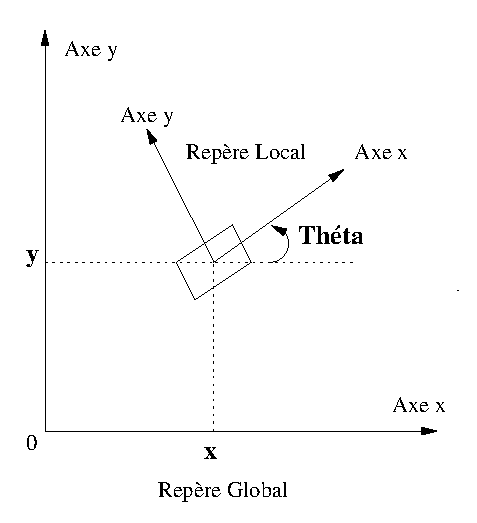
\includegraphics[width=5.8cm]{fig/reperes}
\end{center}
\caption{Description du rep\`ere global et du rep\`ere local associ\'e
\`a un objet graphique}
\end{figure}

\subsection{Rappels sur les {\tt Agent}}

Un {\tt Agent2D} est donc un {\tt Agent},
il a par cons\'equent des possibilit\'es de communication par {\tt Message}
et poss\`ede une m\'ethode {\tt live(double dt)} permettant de
d\'ecrire son comportement.

\begin{center}
Les {\tt Agent2D} sont donc ordonnanc\'es par un {\tt Scheduler}.
\end{center}

%-----------------------------------------------------------------------------

\section{Particularit\'es de la classe {\tt Agent2D}}

Dans cette section, nous d\'ecrivons les fonctionnalit\'es qui
sont propres aux {\tt Agent2D} (i.e. fonctionnalit\'es ne se trouvant
ni dans la classe {\tt Agent}, ni dans la classe {\tt Object2D}).

\vspace{0.3cm}
Rappels~:

\begin{itemize}
\item Un {\tt Agent2D} a donc une position et une orientation puisqu'un
{\tt Agent2D} est un {\tt Object2D}.

\vspace{-0.1cm}
\item Un {\tt Agent2D} a des capacit\'es de d\'etection/perception
puisque c'est un {\tt Object2D}.
Mais attention, un {\tt Agent2D} a ses propres m\'ethodes de
d\'etection/perception...

\vspace{-0.1cm}
\item Les fonctionnalit\'es concernant la gestion d'{\tt Agent}
permettent de conna\^ \i tre tous les {\tt Agent} d'un certain type
(et les types d\'eriv\'es)... voir {\tt getAllAgents}


\noindent
Cela peut-\^etre utile pour qu'un {\tt Agent2D} d\'etecte/per\c coive
les autres {\tt Agent2D}...\\ et
\'eventuellement seulement ceux d'un certain type.
\end{itemize}

\subsection{Vitesses et acc\'el\'erations}

\vspace{0.2cm}
La classe {\tt Agent2D} permet de g\'erer les notions de vitesses
(lin\'eaire et angulaire) et d'acc\'el\'erations (lin\'eaire et angulaire).

\vspace{0.2cm}
Ainsi, en fonction du temps qui passe ({\tt dt}), il
est possible de calculer la nouvelle position/orientation
d'un {\tt Agent2D} connaissant son ancienne position/orientation et ses
vitesses (lin\'eaires et angulaires).
Les nouvelles vitesses (lin\'eaire et angulaire) peuvent \'egalement
\^etre calcul\'ees gr\^ace aux acc\'el\'erations (lin\'eaire et angulaire).

\vspace{0.2cm}
Remarques~:
\begin{itemize}
\item Afin de conna\^ \i tre {\tt dt} et que celui-ci ait un sens,
l'ordonnanceur des {\tt Agent} doit \^etre en mode temps r\'eel
(voir {\tt Scheduler::setRealTimeMode}).
\vspace{-0.1cm}
\item Les {\bf vitesses et acc\'el\'erations lin\'eaires} sont consid\'er\'ees
comme ayant un sens {\bf dans le rep\`ere local} de l'{\tt Agent2D}.
\end{itemize}

\subsubsection{Gestion des vitesses (lin\'eaire et angulaire)}

Dans la classe {\tt Agent2D}, on trouve les m\'ethodes suivantes~:

\begin{itemize}
\item {\tt double getLinearVelocityX(void) const;}
\item {\tt double getLinearVelocityY(void) const;}
\item {\tt double getAngularVelocity(void) const;}
\item {\tt void~~ getVelocity(double\& xVelocity,double\& yVelocity,

~~~~~~~~~~~~~~~~~~~double\& thetaVelocity) const;}
\item {\tt void~~ setLinearVelocityX(double xVelocity);}
\item {\tt void~~ setLinearVelocityY(double yVelocity);}
\item {\tt void~~ setAngularVelocity(double thetaVelocity);}
\item {\tt void~~ setVelocity(double xVelocity,double yVelocity,

~~~~~~~~~~~~~~~~~~~double thetaVelocity);}
\end{itemize}

\subsubsection{Gestion des acc\'el\'erations (lin\'eaire et angulaire)}

Dans la classe {\tt Agent2D}, on trouve les m\'ethodes suivantes~:

\begin{itemize}
\item {\tt double getLinearAccelerationX(void) const;}
\item {\tt double getLinearAccelerationY(void) const;}
\item {\tt double getAngularAcceleration(void) const;}
\item {\tt void~~ getAcceleration(double\& xAcceleration,double\& yAcceleration,

~~~~~~~~~~~~~~~~~~~~~~~double\& thetaAcceleration) const;}
\item {\tt void~~ setLinearAccelerationX(double xAcceleration);}
\item {\tt void~~ setLinearAccelerationY(double yAcceleration);}
\item {\tt void~~ setAngularAcceleration(double thetaAcceleration);}
\item {\tt void~~ setAcceleration(double xAcceleration,double yAcceleration,

~~~~~~~~~~~~~~~~~~~~~~~double thetaAcceleration);}
\end{itemize}

\subsubsection{Calcul cin\'ematique~: {\tt void Kinematic(double dt);}}

Dans la classe {\tt Agent2D} a \'et\'e d\'efinie une m\'ethode
prenant en charge la cin\'ematique~:

\begin{center}
{\tt void Kinematic(double dt);}
\end{center}

Le calcul cin\'ematique effectu\'e permet de g\'erer le d\'eplacement
d'un {\tt Agent2D} en fonction de sa position, de ses vitesses
(lin\'eaire et angulaire) et de ses acc\'el\'erations (lin\'eaire et
angulaire)... et bien s\^ur du temps qui passe {\tt dt}~!

\vspace{0.3cm}
Remarques~:
\begin{itemize}
\item Afin de conna\^ \i tre {\tt dt} et que celui-ci ait un sens,
l'ordonnanceur des {\tt Agent} doit \^etre en mode temps r\'eel
(voir {\tt Scheduler::setRealTimeMode}).
\item La m\'ethode {\tt live(double dt);} des {\tt Agent2D} fait
appel \`a cette m\'ethode {\tt Kinematic}.

\begin{small}
\begin{verbatim}
void Agent2D::live(double dt)
{
 (void)dt; // Pour eviter un warning si pas utilise

 // "Comportement" d'un Agent de la classe Agent2D

 if (dt!=0.0) Kinematic(dt);
}
\end{verbatim}
\end{small}

\item Si par h\'eritage vous d\'erivez de la classe {\tt Agent2D},
il faudra penser \`a faire appel \`a cette m\'ethode {\tt Kinematic}
dans m\'ethode {\tt live} de la classe d\'eriv\'ee.

Et c'est presque magique!
En effet, le fait d'appeler la m\'ethode {\tt Kinematic} permet de voir
un {\tt Agent2D} se d\'eplacer ``tout seul''... en fonction du temps qui
passe {\tt dt}, de ses vitesses (lin\'eaire et angulaire) et
de ses acc\'el\'erations (lin\'eaire et angulaire).
\end{itemize}


\subsection{D\'etections/Perceptions propres aux {\tt Agent2D}}

Un {\tt Agent2D} a des capacit\'es de d\'etection/perception
puisque c'est un {\tt Object2D}.
Mais attention, un {\tt Agent2D} a ses propres m\'ethodes de
d\'etection/perception...

\subsubsection{M\'ethodes de d\'etection/perceptions
de repr\'esentations graphiques\\d'{\tt Agent2D}}

Dans la classe {\tt Agent2D}, on trouve les m\'ethodes suivantes~:

\begin{itemize}
\item \verb|bool /* true: inside, false: outside */| \\
      \verb!isInside(double x, double y) const;!
      \begin{itemize}
      \item Retourne {\tt true} si le point $(x,y)$ est situ\'e \`a
            l'int\'erieur de la repr\'esentation de l'{\tt Agent2D}
            {\tt *this}.
            Retourne {\tt false} sinon.
      \item \verb!x! et \verb!y! sont exprim\'es dans le rep\`ere global.
      \item Cette m\'ethode {\tt isInside} {\bf correspond} \`a celle
            d\'efinie dans la classe {\tt Object2D}.
      \end{itemize}
\item \verb|bool /* true: intersection found, false: no intersection found */|\\
      \verb!intersectRay(double xRay, double yRay, double thetaRay,!\\
      \verb!             double& xOut, double& yOut) const;!
      \begin{itemize}
      \item  Retourne {\tt true} si la repr\'esentation de l'{\tt Agent2D}
             {\tt *this} est intersect\'ee par la demi-droite issue de
             $(xRay,yRay)$ et orient\'ee selon $thetaRay$.
             Retourne {\tt false} sinon.
      \item \verb!xOut! et \verb!yOut! re\c coivent alors le point
            d'intersection.
      \item \verb!xRay!, \verb!yRay!, \verb!thetaRay!, \verb!xOut! et
            \verb!yOut! sont exprim\'es dans le rep\`ere global.
      \item Cette m\'ethode {\tt intersectRay} {\bf correspond}
            \`a celle d\'efinie dans la classe {\tt Object2D}.
      \end{itemize}

\item \verb!Agent2D * /* NULL: no intersection found, not NULL: intersection found */! \\
      \verb!throwRay(double& xOut, double& yOut,! \\
      \verb!         const vector<Agent2D*>& vectAgent2D) const;!
      \begin{itemize}
      \item Lance un rayon devant l'{\tt Agent2D} \verb!*this!
      (via les coordonn\'ees et l'axe de \verb!*this!).
      \item Retourne l'{\tt Agent2D} le plus proche intersect\'e par ce rayon
      ({\tt Agent2D} contenu dans le vecteur \verb!vectAgent2D!, 
      vecteur d'{\tt Agent2D*}).
      \item Retourne \verb!NULL! si pas d'objet intersect\'e.
      \item \verb!xOut! et \verb!yOut! re\c coivent alors le point
      d'intersection.
      \item \verb!xOut! et \verb!yOut! sont exprim\'es dans le rep\`ere global.
      \item Cette m\'ethode {\tt intersectRay} {\bf ne correspond pas}
            \`a celle d\'efinie dans la classe {\tt Object2D}...
            Elle est propre aux {\tt Agent2D}.
      \end{itemize}
\end{itemize}

\subsubsection{M\'ethodes de d\'etection/perception d'{\tt Agent2D}\\
dans un c\^one de vision}

Contrairement aux m\'ethodes de d\'etection de repr\'esentations graphiques
qui travaillent sur les formes 2D des {\tt Agent2D},
les m\'ethodes pr\'esent\'ees dans cette sous-section travaillent sur les
positions ({\tt x},{\tt y}) des {\tt Agent2D}.

\vspace{0.3cm}
Ces m\'ethodes utilisent la notion de c\^one de vision.
Ainsi, pour un {\tt Agent2D}, un c\^one de vision est
d\'etermin\'e par 3 r\'eels {\tt vision}, {\tt range} et {\tt turn}.

\begin{figure}[hbtp]
\begin{center}
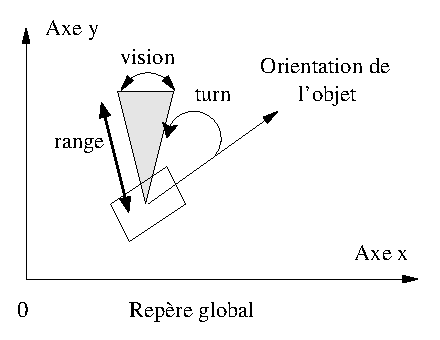
\includegraphics[width=6.5cm]{fig/cone}
\end{center}
\caption{C\^one de d\'etection d'un {\tt Agent2D} en fonction de son
l'orientation et des param\`etres {\tt vision}, {\tt range} et {\tt turn}.
Si {\tt range} est \'egal \`a {\tt 0.0} $\Longrightarrow$ range~: $\infty$.}
\end{figure}

\vspace{0.3cm}
Dans la classe {\tt Agent2D}, on trouve les m\'ethodes suivantes~:

\begin{itemize}
\item \verb!Agent2D * /* NULL: no Agent2D found, not NULL: an Agent2D */!\\
      \verb!viewFirst(string aClass,!\\
      \verb!          double vision, double range, double turn) const;!
      \begin{itemize}
      \item Retourne l'{\tt Agent2D} le plus proche se trouvant dans le
            c\^one de vision de l'{\tt Agent2D} {\tt *this}, c\^one de vision
            d\'etermin\'e par {\tt vision}, {\tt range} et {\tt turn}.
      \item Si {\tt range} est \'egal \`a {\tt 0.0}
            $\Longrightarrow$ range~: $\infty$ 
      \item Seuls les {\tt Agent2D} de la classe {\tt aClass} sont
            per\c cus...

            En interne, il y a un {\tt getAllAgents}~!
      \end{itemize}
\vspace{-0.3cm}
\item \verb!int!\\
      \verb!view(string aClass,!\\
      \verb!     vector<Agent2D*>& vectAgent2D,!\\
      \verb!     double vision, double range, double turn) const;!
      \begin{itemize}
      \item Retourne le nombre d'{\tt Agent2D} se trouvant dans le
            c\^one de vision de l'{\tt Agent2D} {\tt *this},
            c\^one de vision d\'etermin\'e par {\tt vision}, {\tt range}
            et {\tt turn}.
            A la sortie de la m\'ethode, les {\tt Agent2D} se trouvant dans
            ce c\^one de vision sont disponibles dans le vecteur pass\'e
            par r\'ef\'erence ({\tt vectAgent2D}), vecteur d'{\tt Agent2D*}.
      \item Si {\tt range} est \'egal \`a {\tt 0.0}
            $\Longrightarrow$ range~: $\infty$ 
      \item Seuls les {\tt Agent2D} de la classe {\tt aClass} sont
            per\c cus...

            En interne, il y a un {\tt getAllAgents}~!
      \end{itemize}
\vspace{-0.3cm}
\item \verb!Agent2D * /* NULL: no Agent2D found, not NULL: an Agent2D */!\\
      \verb!viewFirstAgent2D(double vision, double range, double turn) const;!
      \begin{itemize}
      \item Revient \`a faire
            {\tt viewFirst("Agent2D",vision,range,turn);}
      \end{itemize}
\vspace{-0.3cm}
\item \verb!int!\\
      \verb!viewAgent2D(vector<Agent2D*>& vectAgent2D,!\\
      \verb!            double vision, double range, double turn) const;!
      \begin{itemize}
      \item Revient \`a faire
            {\tt view("Agent2D",vectAgent2D,vision,range,turn);}
      \end{itemize}
\end{itemize}


\subsection{Pour m\'emoire~: acc\`es aux m\'ethodes de d\'etection/perception\\
de la classe {\tt Object2D}}

Normalement, vous n'avez pas \`a utiliser ces m\'ethodes puisqu'elles sont
disponibles (et sp\'ecialis\'ees) dans la classe {\tt Agent2D}.

\subsubsection{M\'ethodes de d\'etection/perception
de repr\'esentations graphiques\\d'{\tt Object2D}} 

\vspace{0.3cm}
Pour m\'emoire, dans la classe {\tt Object2D},
on trouve les m\'ethodes suivantes~:

\begin{itemize}
\item \verb|bool /* true: inside, false: outside */| \\
      \verb!isInside(double x, double y) const;!
      \begin{itemize}
      \item Retourne {\tt true} si le point $(x,y)$ est situ\'e \`a
            l'int\'erieur de la repr\'esentation de l'{\tt Object2D}
            {\tt *this}.
            Retourne {\tt false} sinon.
      \item \verb!x! et \verb!y! sont exprim\'es dans le rep\`ere global.
      \item Cette m\'ethode {\tt isInside} {\bf correspond}
            \`a celle d\'efinie dans la classe {\tt Agent2D}.
      \end{itemize}
\item \verb|bool /* true: intersection found, false: no intersection found */|\\      \verb!intersectRay(double xRay, double yRay, double thetaRay,!\\
      \verb!             double& xOut, double& yOut) const;!
      \begin{itemize}
      \item  Retourne {\tt true} si la repr\'esentation de l'{\tt Object2D}
             {\tt *this} est intersect\'ee par la demi-droite issue de
             $(xRay,yRay)$ et orient\'ee selon $thetaRay$.
             Retourne {\tt false} sinon.
      \item \verb!xOut! et \verb!yOut! re\c coivent alors le point
            d'intersection.
      \item \verb!xRay!, \verb!yRay!, \verb!thetaRay!, \verb!xOut! et
            \verb!yOut! sont exprim\'es dans le rep\`ere global.
      \item Cette m\'ethode {\tt intersectRay} {\bf correspond}
            \`a celle d\'efinie dans la classe {\tt Agent2D}.
      \end{itemize}
\item \verb!Object2D * /* NULL: no intersection found, not NULL: intersection found */! \\
      \verb!throwRay(double& xOut, double& yOut,! \\
      \verb!         Object2D *tabObject2D[], unsigned int nbObject2D) const;!
      \begin{itemize}
      \item Lance un rayon devant l'{\tt Object2D} \verb!*this!
      (via les coordonn\'ees et l'axe de \verb!*this!).
      \item Retourne l'{\tt Object2D} le plus proche intersect\'e par ce
      rayon ({\tt Object2D} contenu dans le tableau \verb!tabObject2D!,
      tableau de {\tt nbObject2D} \'el\'ements de type {\tt Object2D*}).
      \item Retourne \verb!NULL! si pas d'objet intersect\'e.
      \item \verb!xOut! et \verb!yOut! re\c coivent alors le point
      d'intersection.
      \item \verb!xOut! et \verb!yOut! sont exprim\'es dans le rep\`ere global.
      \item Cette m\'ethode {\tt intersectRay} {\bf ne correspond pas}
            \`a celle d\'efinie dans la classe {\tt Agent2D}...
            Elle est propre aux {\tt Object2D}.
      \end{itemize}
\end{itemize}

\subsubsection{M\'ethodes de d\'etection/perception d'{\tt Object2D}\\
dans un c\^one de vision}

\vspace{0.2cm}
Contrairement aux fonctions de d\'etection de repr\'esentations graphiques
qui travaillent sur les formes 2D des objets, les fonctions pr\'esent\'ees
dans cette sous-section travaillent sur les positions ({\tt x},{\tt y}) des
objets.

\vspace{0.4cm}
Ces fonctions utilisent la notion de c\^one de vision.
Ainsi, pour un {\tt Object2D}, un c\^one de vision est
d\'etermin\'e par 3 r\'eels {\tt vision}, {\tt range} et {\tt turn}.

\vspace{0.2cm}
\begin{figure}[hbtp]
\begin{center}
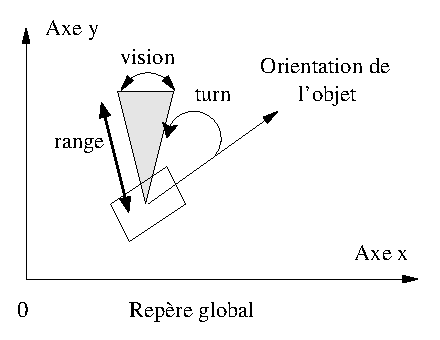
\includegraphics[width=6.5cm]{fig/cone}
\end{center}
\caption{C\^one de d\'etection d'un object en fonction de son l'orientation
et des param\`etres {\tt vision}, {\tt range} et {\tt turn}.
Si {\tt range} est \'egal \`a {\tt 0.0} $\Longrightarrow$ range~: $\infty$.}
\end{figure}

Pour m\'emoire, dans la classe {\tt Object2D},
on trouve les m\'ethodes suivantes~:

\vspace{0.2cm}
\begin{itemize}
\item \verb!Object2D * /* NULL: no Object2D found, not NULL: an Object2D */!\\
      \verb!viewFirstObject2D(double vision, double range, double turn) const;!
      \begin{itemize}
      \item Retourne l'{\tt Object2D} le plus proche se trouvant dans le
            c\^one de vision de l'{\tt Object2D} {\tt *this},
            c\^one de vision d\'etermin\'e par {\tt vision}, {\tt range} et
            {\tt turn}.
      \item Si {\tt range} est \'egal \`a {\tt 0.0}
            $\Longrightarrow$ range~: $\infty$ 
      \end{itemize}
\vspace{0.2cm}
\item \verb!int!\\
      \verb!viewObject2D(vector<Object2D*>& vectObject2D,!\\
      \verb!             double vision, double range, double turn) const;!
      \begin{itemize}
      \item Retourne le nombre d'{\tt Object2D} se trouvant dans le
            c\^one de vision de l'{\tt Object2D} {\tt *this},
            c\^one de vision d\'etermin\'e par {\tt vision}, {\tt range}
            et {\tt turn}.
            A la sortie de la m\'ethode, les {\tt Object2D} se trouvant dans
            ce c\^one de vision sont disponibles dans le vecteur pass\'e
            par r\'ef\'erence ({\tt vectObject2D}), vecteur d'{\tt Object2D*}.
      \item Si {\tt range} est \'egal \`a {\tt 0.0}
            $\Longrightarrow$ range~: $\infty$ 
      \end{itemize}
\end{itemize}

\subsubsection{Utilisation~: attention \`a l'h\'eritage multiple~!}

Si vous d\'ecidez d'utiliser ces m\'ethodes de la classe {\tt Object2D},
il faut faire attention \`a l'h\'eritage multiple ayant permis
d'obtenir la classe {\tt Agent2D} \`a partir de la classe {\tt Agent}
et de la classe {\tt Object2D}.

\newpage

Soit l'exemple suivant~:

\begin{small}
\begin{verbatim}
   // La classe Petit heritant de la classe Agent2D
   // La classe Poisson heritant de la classe Agent2D
   .....
   vector<Agent*> v;
   getAllAgents("Petit",v);
   int nbAgents=v.size();

   Object2D* unObject2D = (Agent2D*)getAgent("Poisson.1");

   Object2D** tab = (Object2D**)malloc(nbAgents*sizeof(Object2D*));

   // v : vecteur d'Agent*
   // tab : tableau d'Object2D*
   for(int i=0;i<nbAgents;i++)
   {
    tab[i]=(Agent2D*)v[i]; // Ecrire tab[i]=(Object2D*)v[i]; est une erreur !
   }

   double x,y;
   Object2D* objFound=unObject2D->throwRay(x,y,tab,nbAgents);

   if (objFound!=NULL) objFound->setColor("yellow");

   free(tab);
   .....
\end{verbatim}
\end{small}

Sur cet exemple, nous constatons qu'il n'est pas possible, \`a cause
de l'h\'eritage multiple, de passer d'un {\tt Agent*} \`a un {\tt Object2D*}
directement... Il faut passer par {\tt Agent2D*}~!

\vspace{0.3cm}
$\Longrightarrow$ Le mieux est certainement d'utiliser les m\'ethodes
de d\'etection/perception de la classe

\hspace{0.8cm}{\tt Agent2D}~!

%---------------------------------------------------------------

\section{Initialisation, activation et param\'etrage de\\
         l'application graphique}

En plus de l'interface de la classe {\tt Agent2D},
le fichier

\vspace{-0.3cm}
\begin{center}
\verb!GestionAgents2D/LibAgents2D/include/Agent2D.h!
\end{center}

\vspace{-0.3cm}
donne \'egalement acc\`es \`a des fonctions
permettant d'initialiser et d'activer l'application graphique~:

\vspace{-0.2cm}
\begin{itemize}
\item \verb!void! \\
      \verb!graphic_init(const char * windowName,! \\
      \verb!             const char * fontName);!
      \begin{itemize}
      \item Cr\'eer la fen\^etre graphique en lui affectant le titre
            \verb!windowName!.
\vspace{-0.2cm}
      \item Les \verb!Agent2D!s ayant une repr\'esentation sous forme
            de texte utiliseront la police \verb!fontName!.
\vspace{-0.2cm}
      \item Cette fonction doit \^etre appel\'ee avant toutes les autres
            fonctions de la bi\-blio\-th\`eque.
      \end{itemize}
\item \verb!void! \\
      \verb!graphic_setWidth(int width);!
      \begin{itemize}
      \item Fixer la largeur en pixels de la fen\^etre graphique.
      \end{itemize}
\item \verb!void! \\
      \verb!graphic_setHeight(int height);!
      \begin{itemize}
      \item Fixer la hauteur en pixels de la fen\^etre graphique.
      \end{itemize}
\item \verb!void! \\
      \verb!graphic_setBackground(const char * colorName);!
      \begin{itemize}
      \item Changer la couleur du fond de la fen\^etre graphique.
      \end{itemize}
\item \verb!void! \\
      \verb!graphic_setViewPoint(double x,! \\
      \verb!                     double y,! \\
      \verb!                     double scale);!
      \begin{itemize}
      \item Modifier le point de vue de la fen\^etre
      \item Le point $(x,y)$ repr\'esente le point du plan qui sera situ\'e
            au centre de la fen\^etre.
      \item \verb!scale! repr\'esente le facteur qui permet de passer des
            grandeurs sans dimension du plan aux \textit{pixels} de l'\'ecran.
      \end{itemize}
\item \verb!void! \\
      \verb!graphic_getViewPoint(double * xOut,! \\
      \verb!                     double * yOut,! \\
      \verb!                     double * scaleOut);!
      \begin{itemize}
      \item Obtenir le point de vue courant de la fen\^etre.
      \item Voir \verb!graphic_setViewPoint()! .
      \end{itemize}
\item \verb!void! \\
      \verb!graphic_autoscale(void);!
      \begin{itemize}
      \item Recadrer la fen\^etre pour qu'elle montre
            l'ensemble des \verb!Agent2D!s.
      \end{itemize}
\item \verb!void! \\
      \verb!graphic_run(void * userData);!
      \begin{itemize}
      \item Lancer la partie active (\'ev\'enementielle) du programme.
      \item \verb!userData! d\'esigne g\'en\'eralement une structure
            cr\'e\'ee par vos soins, permettant d'acc\'eder \`a l'ensemble
            des donn\'ees de l'application.
      \end{itemize}
\item \verb!void! \\
      \verb!graphic_mainLoop(void * userData);!
      \begin{itemize}
      \item Cette fonction est appel\'ee perp\'etuellement \`a partir
            de \verb!graphic_run()!~; c'est le c\oe ur de l'application.
      \item \textbf{Vous devez d\'efinir cette fonction !}
      \item Le param\`etre \verb!userData! est celui qui a \'et\'e
            transmis \`a \verb!graphic_run()!.
      \end{itemize}
\item \verb!void! \\
      \verb!graphic_keyPressCallback(Agent2D * agt2d,! \\
      \verb!                         const char * key,! \\
      \verb!                         void * userData);!
      \begin{itemize}
      \item Cette fonction est appel\'ee lorsqu'une touche du clavier est
            enfonc\'ee.
      \item \textbf{Vous devez d\'efinir cette fonction !}
      \item Si \verb!agt2d! est non nul, il s'agit d'un objet graphique
            qui \'etait s\'electionn\'e lors de l'appui sur la touche.
      \item Si \verb!agt2d! est nul, aucun objet graphique n'\'etait
            s\'electionn\'e au moment de l'appui sur la touche.
      \item La touche enfonc\'ee est d\'ecrite de mani\`ere lisible par
            \verb!key!.
      \item Le param\`etre \verb!userData! est celui qui a \'et\'e
            transmis \`a \verb!graphic_run()!.
      \end{itemize}
\item \verb!void! \\
      \verb!graphic_mouseDragCallback(Object2D * agt2d,! \\
      \verb!                          double dx, double dy,! \\
      \verb!                          void * userData);!
      \begin{itemize}
      \item Cette fonction est appel\'ee lorsqu'un mouvement de souris
            est appliqu\'e \`a un \verb!Agent2D!.
      \item \textbf{Vous devez d\'efinir cette fonction !}
      \item \verb!agt2d! d\'esigne l'objet s\'electionn\'e lors du
            mouvement de souris.
      \item Le mouvement est d\'ecrit par le vecteur $(dx,dy)$ dans le
            rep\`ere global.
      \item Le param\`etre \verb!userData! est celui qui a \'et\'e
            transmis \`a \verb!graphic_run()!.
      \end{itemize}
\end{itemize}

Tous les mouvements et les dimensions des \verb!Agent2D! sont exprim\'es
dans une grandeur sans dimention~; ce ne sont pas des pixels.
L'axe $\vec{x}$ cro{\^\i}t de gauche \`a droite et l'axe $\vec{y}$ de bas
en haut. Le point de vue de la fen\^etre peut \^etre modifi\'e selon des
translations (\verb!Ctrl!+Click Gauche) et selon un facteur de grossissement
(\verb!Ctrl!+Click Droit).

\vspace{-0.1cm}
\section{Programme minimal}

\vspace{-0.1cm}
Cette section pr\'esente un programme minimal permettant de
g\'erer des {\tt Agent2D}~: gestion d'un ordonnanceur + application
graphique (voir {\tt GestionAgents2D/Exemples/prgMinimal})

\vspace{-0.1cm}
\begin{small}
\begin{verbatim}
#ifndef _APPLIDATA_H           /* Fichier : AppliData.h */
#define _APPLIDATA_H

#include "Agent2D.h"

typedef struct
{
Scheduler* sched;
Agent2D*   obj;
int        autoscale;
int        pause;
} AppliData;

#endif // _APPLIDATA_H
\end{verbatim}
\end{small}

\begin{small}
\begin{verbatim}
#include "Agent2D.h"             /* Fichier : prg.cpp */

/*------------------------------ Application --------------------------------*/
/*---- application specific data ----*/
\end{verbatim}
\vspace{-0.4cm}
\begin{verbatim}
#include "AppliData.h"
\end{verbatim}
\vspace{-0.4cm}
\begin{verbatim}
void deleteAppliData(AppliData * data)
{
 delete(data->obj);
 delete(data->sched);
 delete(data);
}
\end{verbatim}
\vspace{-0.4cm}
\begin{verbatim}
void help(void)
{
 cout << "*********************************************"<< endl;
 cout << "help"                                         << endl;
 cout << "----"                                         << endl;
 cout << "Actions clavier AVEC objet selectionne:"      << endl;
 cout << "- p : obtenir le nom d'un Agent2D"            << endl;
 cout << "Actions clavier SANS objet selectionne:"      << endl;
 cout << "- h : help"                                   << endl;
 cout << "- a : autoscale (oui/non)"                    << endl;
 cout << "-' ': pause     (oui/non)"                    << endl;
 cout << "- q : quitter"                                << endl;
 cout << "*********************************************"<< endl;
}
\end{verbatim}
\vspace{-0.4cm}
\begin{verbatim}
int main(void)
{
AppliData * data;
\end{verbatim}
\vspace{-0.4cm}
\begin{verbatim}
/*---- initialize graphic window ----*/
\end{verbatim}
\vspace{-0.4cm}
\begin{verbatim}
graphic_init("My Window","-*-helvetica-*-r-normal--14-*");
graphic_setWidth(640);
graphic_setHeight(480);
graphic_setBackground("cyan4");
\end{verbatim}
\vspace{-0.4cm}
\begin{verbatim}
/*---- initialize application specific data ----*/
\end{verbatim}
\vspace{-0.4cm}
\begin{verbatim}
data=(AppliData *)malloc(sizeof(AppliData));
data->sched=new Scheduler;
data->sched->setRealTimeMode(true);
\end{verbatim}
\vspace{-0.4cm}
\begin{verbatim}
/*---- initialize Agent2D  ----*/
\end{verbatim}
\vspace{-0.4cm}
\begin{verbatim}
data->obj=new Agent2D();
data->obj->square(10,0);
data->obj->setAngularVelocity(1); // Vitesse angulaire
\end{verbatim}
\begin{verbatim}
/*----- initialize specific data -----*/
\end{verbatim}
\vspace{-0.4cm}
\begin{verbatim}
data->autoscale=1;
data->pause=0;
\end{verbatim}
\newpage
\begin{verbatim}
/*---- run the graphic application ----*/
\end{verbatim}
\vspace{-0.6cm}
\begin{verbatim}
help();
\end{verbatim}
\vspace{-0.6cm}
\begin{verbatim}
graphic_run(data);
return(0);
}
\end{verbatim}
\vspace{-0.6cm}
\begin{verbatim}
void
graphic_mainLoop(void * userData)
{
AppliData * data=(AppliData *)userData;
if(!data->pause)
  {
   data->sched->cycle();   // Lancement d'un cycle de l'ordonnanceur
  }
if(data->autoscale)
  {
   graphic_autoscale();
  }
}
\end{verbatim}
\vspace{-0.6cm}
\begin{verbatim}
void
graphic_keyPressCallback(Agent2D * agt2d,
                         const char * key,
                         void * userData)
{
AppliData * data=(AppliData *)userData;
(void)data;
\end{verbatim}
\vspace{-0.6cm}
\begin{verbatim}
if (agt2d==NULL)         // Interaction clavier SANS objet selectionne
{
 if(!strcmp(key,"Left"))
  {
  graphic_mouseDragCallback(data->obj,
                            -0.5,0.0,userData); // simulate mouse drag
  }
 else if(!strcmp(key,"Right"))
  {
  graphic_mouseDragCallback(data->obj,
                            0.5,0.0,userData); // simulate mouse drag
  }
 else if(!strcmp(key,"h")||!strcmp(key,"H"))
  {
  help();
  }
 else if(!strcmp(key,"a")||!strcmp(key,"A"))
  {
  data->autoscale=1-data->autoscale;
  }
 else if(!strcmp(key," "))
  {
  data->pause=1-data->pause;
  }
\end{verbatim}
\newpage
\begin{verbatim}
 else if(!strcmp(key,"q")||!strcmp(key,"Q")||!strcmp(key,"\x1b")) // Esc
  {
  deleteAppliData(data);
  exit(0);
  }
 else { fprintf(stderr,"Viewer key <%s>\n",key); }
 return;
}
        //  ET donc ici, interaction clavier AVEC un objet selectionne
\end{verbatim}
\vspace{-0.6cm}
\begin{verbatim}
agt2d->onKeyPress(key);  // Par defaut : si p affiche le nom de l'Agent2D
}
\end{verbatim}
\vspace{-0.6cm}
\begin{verbatim}
void
graphic_mouseDragCallback(Agent2D * agt2d,
                          double dx,
                          double dy,
                          void * userData)
{
AppliData * data=(AppliData *)userData;
(void)data;
\end{verbatim}
\vspace{-0.6cm}
\begin{verbatim}
agt2d->onMouseDrag(dx,dy); // Par defaut : deplacement de l'Agent2D a la souris
}
\end{verbatim}
\end{small}

\vspace{-0.4cm}
\section{Co--existence {\tt Agent2D}/{\tt Object2D}}

\vspace{-0.1cm}
Les {\tt Agent2D} \'etant des objets graphiques avec un comportement,
il est pr\'ef\'erable de d\'ecrire les \'el\'ements de d\'ecor
(i.e. sans comportement) \`a l'aide d'{\tt Object2D}.

\vspace{0.2cm}
Cela peut poser quelques probl\`emes vis-\`a-vis des interactions
avec la souris ou le clavier.

\vspace{0.2cm}
Reprenons le programme minimal d\'ecrit lors de la section
pr\'ec\'edente. Celui-ci doit \^etre modifi\'e de fa\c con 
\`a g\'erer la co--existence entre les {\tt Agent2D} et
les {\tt Object2D}.

\vspace{0.2cm}
Nous introduisons pour cela la notion de d\'ecor o\`u,
tous les {\tt Object2D} doivent \^etre ajouter afin de
g\'erer correctement l'interaction souris/clavier.

\vspace{0.2cm}
Le fichier {\tt decor.h} ci--apr\`es
d\'ecrit le type {\tt Decor}.
Attention~:~vous n'avez pas a d\'eclarer d'objet
de ce type.
Il en existe d\'ej\`a un d\'eclar\'e dans la biblioth\`eque~!...
et le fichier {\tt decor.h} d\'ecrit les op\'erations
possibles sur cet objet.

\begin{small}
\begin{verbatim}
#ifndef  _DECOR_H_                     /* Fichier : decor.h */
#define  _DECOR_H_
\end{verbatim}
\begin{verbatim}
#include <set>
#include "Object2D.h"
\end{verbatim}
\begin{verbatim}
using namespace std;
\end{verbatim}
\begin{verbatim}
typedef set<Object2D*> Decor;
\end{verbatim}
\begin{verbatim}
extern Decor decor;       // Contient uniquement des Object2D pas des Agent2D !
\end{verbatim}
\begin{verbatim}
extern void addDecor(Object2D* obj2d);    // Ajouter un element du decor
extern void removeDecor(Object2D* obj2d); // Enlever un element du decor
extern bool isInDecor(Object2D* obj2d); // Tester si un objet est dans le decor
\end{verbatim}
\begin{verbatim}
#endif //_DECOR_H_
\end{verbatim}
\end{small}

\newpage
L'id\'ee est ici d'ajouter des \'el\'ements au d\'ecor
(tous les {\tt Object2D} de l'environnement).
Ensuite, lors d'une interaction,
il suffit de tester si l'objet ayant subit l'interaction est dans le d\'ecor.
S'il est dans le d\'ecor, c'est un {\tt Object2D}. Sinon,
c'est un {\tt Agent2D}.
Ce test doit \^etre fait dans les fonctions
{\tt graphic\_keyPressCallback} et {\tt graphic\_mouseDragCallback}.


\vspace{0.4cm}
Les modifications a apporter au programme minimal
(d\'ecrit dans la section pr\'ec\'edente) sont indiqu\'ees via
des commentaires {\tt // *** AJOUT ..! *** }.

\begin{small}
\begin{verbatim}

#ifndef _APPLIDATA_H          /* Fichier AppliData.h */
#define _APPLIDATA_H

#include "Agent2D.h"
#include "Object2D.h"

typedef struct
{
Scheduler* sched;
Agent2D*   agt;
Object2D*  obj;               // *** AJOUT ..! ***
int        autoscale;
int        pause;
} AppliData;
#endif // _APPLIDATA_H
\end{verbatim}
\end{small}

Et maintenant le fichier {\tt prg.cpp}

\begin{small}
\begin{verbatim}

/*----------------------------------------------------------------------------
  prg.cpp
----------------------------------------------------------------------------*/

#include "Agent2D.h"

#include "Decor.h"            // *** AJOUT ..! *** 
#include "Object2D.h"         // *** AJOUT ..! ***

/*-------- Application -----------------------------------------------------*/

/*---- application specific data ----*/

#include "AppliData.h"

void deleteAppliData(AppliData * data)
{
 removeDecor(data->obj);      // *** AJOUT ..! ***
 delete(data->obj);
 delete(data->agt);
 delete(data->sched);
 delete(data);
}


void help(void)
{
 cout << "*********************************************"<< endl;
 cout << "help"                                         << endl;
 cout << "----"                                         << endl;
 cout << "Actions clavier AVEC objet selectionne:"      << endl;
 cout << "- p : obtenir le nom d'un Agent2D"            << endl;
 cout << "Actions clavier SANS objet selectionne:"      << endl;
 cout << "- h : help"                                   << endl;
 cout << "- a : autoscale (oui/non)"                    << endl;
 cout << "-' ': pause     (oui/non)"                    << endl;
 cout << "- q : quitter"                                << endl;
 cout << "*********************************************"<< endl;
}

int
main(void)
{
AppliData * data;
\end{verbatim}
\begin{verbatim}
/*---- initialize graphic window ----*/
\end{verbatim}
\begin{verbatim}
graphic_init("My Window","-*-helvetica-*-r-normal--14-*");
graphic_setWidth(640);
graphic_setHeight(480);
graphic_setBackground("cyan4");
\end{verbatim}
\begin{verbatim}
/*---- initialize application specific data ----*/
\end{verbatim}
\begin{verbatim}
data=(AppliData *)malloc(sizeof(AppliData));
data->sched=new Scheduler;
data->sched->setRealTimeMode(true);
\end{verbatim}
\begin{verbatim}
/*---- initialize Agent2D  ----*/
\end{verbatim}
\begin{verbatim}
data->agt=new Agent2D();
data->agt->square(10,0);
data->agt->setAngularVelocity(1);
\end{verbatim}
\begin{verbatim}
data->obj=new Object2D();          // *** AJOUT ..! ***
addDecor(data->obj);               // *** AJOUT ..! ***
data->obj->square(15,0);           // *** AJOUT ..! ***
data->agt->attachTo(*data->obj);   // *** AJOUT ..! ***
\end{verbatim}
\begin{verbatim}
/*----- initialize specific data -----*/
\end{verbatim}
\begin{verbatim}
data->autoscale=1;
data->pause=0;
\end{verbatim}
\begin{verbatim}
/*---- run the graphic application ----*/
\end{verbatim}
\begin{verbatim}
help();
\end{verbatim}
\begin{verbatim}
graphic_run(data);
return(0);
}
\end{verbatim}
\newpage
\begin{verbatim}
void
graphic_mainLoop(void * userData)
{
AppliData * data=(AppliData *)userData;
if(!data->pause)
  {
   data->sched->cycle(); // Lancement d'un cycle de l'ordonnanceur
  }
if(data->autoscale)
  {
   graphic_autoscale();
  }
}
\end{verbatim}
\begin{verbatim}
void
graphic_keyPressCallback(Agent2D * agt2d,
                         const char * key,
                         void * userData)
{
AppliData * data=(AppliData *)userData;
(void)data;
\end{verbatim}
\begin{verbatim}
if (agt2d==NULL)         // Interaction clavier SANS objet selectionne
{
 if(!strcmp(key,"Left"))
  {
  graphic_mouseDragCallback(data->agt,
                            -0.5,0.0,userData); // simulate mouse drag
  }
 else if(!strcmp(key,"Right"))
  {
  graphic_mouseDragCallback(data->agt,
                            0.5,0.0,userData); // simulate mouse drag
  }
 else if(!strcmp(key,"h")||!strcmp(key,"H"))
  {
  help();
  }
 else if(!strcmp(key,"a")||!strcmp(key,"A"))
  {
  data->autoscale=1-data->autoscale;
  }
 else if(!strcmp(key," "))
  {
  data->pause=1-data->pause;
  }
 else if(!strcmp(key,"q")||!strcmp(key,"Q")||!strcmp(key,"\x1b")) // Esc
  {
  deleteAppliData(data); exit(0);
  }
 else { fprintf(stderr,"Viewer key <%s>\n",key); }
 return;
}
\end{verbatim}
\newpage
\begin{verbatim}
        //  ET donc ici, interaction clavier AVEC un objet selectionne

if (isInDecor((Object2D*)agt2d))                 // *** AJOUT ..! ***
{// Interaction avec les Object2D du decor       // *** AJOUT ..! ***
 Object2D* obj2d=(Object2D*)agt2d;               // *** AJOUT ..! ***
 obj2d->onKeyPress(key);                         // *** AJOUT ..! ***
 return;                                         // *** AJOUT ..! ***
}                                                // *** AJOUT ..! ***

agt2d->onKeyPress(key); // Par defaut : si p affiche le nom de l'Agent2D
}

void
graphic_mouseDragCallback(Agent2D * agt2d,
                          double dx,
                          double dy,
                          void * userData)
{
AppliData * data=(AppliData *)userData;
(void)data;

if (isInDecor((Object2D*)agt2d))                 // *** AJOUT ..! ***
{// Interaction avec les Object2D du decor       // *** AJOUT ..! ***
 Object2D* obj2d=(Object2D*)agt2d;               // *** AJOUT ..! ***
 obj2d->onMouseDrag(dx,dy);                      // *** AJOUT ..! ***
 return;                                         // *** AJOUT ..! ***
}                                                // *** AJOUT ..! ***

agt2d->onMouseDrag(dx,dy); // Par defaut : deplacement de l'Agent2D a la souris
}

/*--------------------------------------------------------------------------*/
\end{verbatim}
\end{small}

\section{Interface public/protected de la classe {\tt Agent2D}}

\begin{center}
{\bf Fichier : {\tt GestionAgents2D/LibAgents2D/include/Agent2D.h}}
\end{center}

\vspace{-0.4cm}
\begin{small}
\begin{verbatim}
class Agent2D : public Agent,
                public Object2D
{
  DEFCLASS(Agent2D)
\end{verbatim}
\begin{verbatim}
  friend ostream& operator<<(ostream& os, const Agent2D& anA);
\end{verbatim}
\begin{verbatim}
 public :
\end{verbatim}
\begin{verbatim}
   // Allocateurs/Desallocateurs
\end{verbatim}
\begin{verbatim}
            Agent2D(void);
            Agent2D(const Agent2D& anA);
            Agent2D& operator=(const Agent2D& anA);
   virtual ~Agent2D(void);

   virtual  void live(double dt);
                                                    // Par defaut :
   virtual  void onKeyPress(const char * key);      // si p affiche le nom
   virtual  void onMouseDrag(double dx, double dy); // deplacement souris

   // Comparaisons

   friend  bool operator==(const Agent2D& anA1, const Agent2D& anA2);
   friend  bool operator!=(const Agent2D& anA1, const Agent2D& anA2);

   // Inspecteurs/modificateurs

      ///////////////////////////////////////////////
      // En plus, ... Voir Agent.h et Object2D.h ...!
      ///////////////////////////////////////////////

      // Gestion de la cinematique :
      // ---------------------------

      void   Kinematic(double dt);  // Modification de la position/orientation

      // Velocity: xVelocity, yVelocity, thetaVelocity
      // ---------------------------------------------

      double getLinearVelocityX(void) const;
      double getLinearVelocityY(void) const;
      double getAngularVelocity(void) const;
      void   getVelocity(double& xVelocity,double& yVelocity,
                         double& thetaVelocity) const;

      void   setLinearVelocityX(double xVelocity);
      void   setLinearVelocityY(double yVelocity);
      void   setAngularVelocity(double thetaVelocity);
      void   setVelocity(double xVelocity,double yVelocity,
                         double thetaVelocity);

      // Acceleration xAcceleration, yAcceleration, thetaAcceleration
      // ------------------------------------------------------------

      double getLinearAccelerationX(void) const;
      double getLinearAccelerationY(void) const;
      double getAngularAcceleration(void) const;
      void   getAcceleration(double& xAcceleration,double& yAcceleration,
                             double& thetaAcceleration) const;

      void   setLinearAccelerationX(double xAcceleration);
      void   setLinearAccelerationY(double yAcceleration);
      void   setAngularAcceleration(double thetaAcceleration);
      void   setAcceleration(double xAcceleration,double yAcceleration,
                             double thetaAcceleration);

   // Perception/Detection

   bool   isInside(double x, double y) const;
   bool   intersectRay(double xRay, double yRay, double thetaRay,
                       double& xOut, double& yOut) const;
   Agent2D * throwRay(double& xOut, double& yOut,
                      const vector<Agent2D*>& vectAgent2D) const;

   Agent2D * viewFirst(string aClass,
                       double vision, double range,
                       double turn=0.0) const;

   int       view(string aClass, vector<Agent2D*>& vectAgent2D,
                  double vision, double range,
                  double turn=0.0) const;

   Agent2D * viewFirstAgent2D(double vision, double range,
                              double turn=0.0) const;

   int       viewAgent2D(vector<Agent2D*>& vectAgent2D,
                         double vision, double range,
                         double turn=0.0) const;

 protected :

   // Methodes a appeler par une classe derivee

   // display: a appeler dans une classe derivee      // display est une
   virtual void display(ostream& os) const;           // methode appelee
                                                      // dans operator<<

   // isEqualTo: a appeler dans une classe derivee (dans operator==)
   virtual bool isEqualTo(const Agent2D& anA) const;
};

/*-------- Graphical application template ----------------------------------*/

extern void graphic_init(const char * windowName, const char * fontName);

extern void graphic_setWidth(int width);

extern void graphic_setHeight(int height);

extern void graphic_setBackground(const char * colorName);

extern void graphic_setViewPoint(double x, double y, double scale);

extern void graphic_getViewPoint(double * xOut, double * yOut,
                                 double *scaleOut);

extern void graphic_autoscale(void);

extern void graphic_run(void * userData);

extern void graphic_mainLoop(void * userData);

extern void graphic_keyPressCallback(Agent2D * agt2d,
                                     const char * key,
                                     void * userData);

extern void graphic_mouseDragCallback(Agent2D * agt2d,
                                      double dx, double dy,
                                      void * userData);

/*-------- Graphical application template --------*/
/*
   int
   main(void)
   {
   graphic_init("My Window","-*-helvetica-*-r-normal--14-*");
   graphic_setWidth(640);
   graphic_setHeight(480);
   ... application specific initializations ...
   graphic_run(myDataPointer);
   return(0);
   }

   void
   graphic_mainLoop(void * userData)
   {
   ...
   }

   void
   graphic_keyPressCallback(Agent2D * agt2d,
                            const char * key,
                            void * userData)
   {
   ...
   }

   void
   graphic_mouseDragCallback(Agent2D * agt2d,
                             double dx,
                             double dy,
                             void * userData)
   {
   ...
   }
*/
\end{verbatim}
\end{small}

\section{Pour m\'emoire~:\\
Interface {\tt public/protected} de la classe {\tt Agent}}

\begin{center}
{\bf Fichier : {\tt GestionAgents/LibMoRis/include/Agent.h}}
\end{center}

\vspace{0.1cm}
Dans {\tt GestionAgents/LibMoRis/include},\\
il faut voir \'egalement la classe {\tt Scheduler} et la classe
{\tt Message}~!

\vspace{0.3cm}
\begin{small}
\begin{verbatim}
typedef void (Agent::*liveMethodType)(double dt); // Pour get/setLiveMethod...

class Agent {
\end{verbatim}
\begin{verbatim}
 DEFCLASS(Agent)
\end{verbatim}
\begin{verbatim}
  friend ostream& operator<<(ostream& os, const Agent& anAgent);
\end{verbatim}
\begin{verbatim}
 public:
\end{verbatim}
\begin{verbatim}
   // Allocateurs/Desallocateurs
\end{verbatim}
\begin{verbatim}
           Agent(void);
           Agent(const Agent& anAgent);
           Agent& operator=(const Agent& anAgent);
  virtual ~Agent(void);
\end{verbatim}
\begin{verbatim}
  virtual  void live(double dt)               // dt en seconde : temps depuis
           {                                  // la derniere activation
            // Rien pour un Agent de base
            (void)dt;  // Pour eviter un warning
           }
\end{verbatim}
\begin{verbatim}
           void suspend(void);
           void restart(void);
           bool isSuspended(void) const;
\end{verbatim}
\begin{verbatim}
           void setLiveMethod(liveMethodType newLiveMethod); // Progr. avertis!
           liveMethodType getLiveMethod(void);               // Progr. avertis!
\end{verbatim}
\begin{verbatim}
   // Comparaisons
\end{verbatim}
\begin{verbatim}
  friend   bool operator==(const Agent& anAgent1, const Agent& anAgent2);
  friend   bool operator!=(const Agent& anAgent1, const Agent& anAgent2);
\end{verbatim}
\begin{verbatim}
   // Inspecteurs
\end{verbatim}
\begin{verbatim}
           string getName(void) const;  // N'a pas de sens dans le constructeur 
           unsigned long getSuffix(void) const; // Idem : n'a pas de sens ...
           string getClass(void) const; // DEFCLASS: virtual getClassName ... 
           bool   isA(string aClass) const;
\end{verbatim}
\begin{verbatim}
   // Gestion des messages
\end{verbatim}
\begin{verbatim}
           size_t   getNbMessages(void) const;
           Message* getNextMessage(void); // Le suivant
           void     clearMessageBox(void);

           void     setSensitivity(string aClass,bool yesNo);
                                                                 // retourne
   virtual size_t   sendMessageTo(Message& aM,Agent *dest) const;// 1(ok),0(ko)
   virtual void     broadcastMessage(Message& aM) const;
\end{verbatim}
\newpage
\begin{verbatim}



 protected:

   // Methodes a appeler par une classe derivee

                                // Methode qui doit etre appelee dans le cons-
           void newAgent(void); // tructeur d'une classe derivee
                                // => Arbre d'heritage

           void newAgent(Agent* This); // Idem mais pour l'heritage multiple
                                       // ... pour programmeurs avertis !

   //  display a appeler dans une classe derivee       // display est une
   virtual void display(ostream& os) const;            // methode appelee
                                                       // dans operator<<

   //  isEqualTo a appeler dans une classe derivee     // isEqualTo est une
   virtual bool isEqualTo(const Agent& anAgent) const; // methode appelee
                                                       // dans operator==
};
\end{verbatim}
\end{small}

\section{Pour m\'emoire~:\\
Interface publique de la classe {\tt Object2D}}

\begin{center}
{\bf Fichier : {\tt GestionObjects2D/LibObjects2D/include/Object2D.h}}
\end{center}

\begin{small}
\begin{verbatim}
class Object2D
{
 friend ostream& operator<<(ostream& os, const Object2D& object2D);

 public :

/*-------- Constructor/Destructor -----------------------------------------*/

         Object2D(void);
         Object2D(const Object2D& object2D);
virtual ~Object2D(void);

         Object2D& operator=(const Object2D& object2D);

 // Test d'egalite uniquement sur la couleur et le type de forme:
 // noShape, point, text, 
 friend   bool operator==(const Object2D& obj1, const Object2D& obj2);
 friend   bool operator!=(const Object2D& obj1, const Object2D& obj2);

/*-------- Location -------------------------------------------------------*/

      void   setLocation(double x, double y, double theta);
      void   getLocation(double& xOut, double& yOut, double& thetaOut) const;
      void   setX(double x);
      double getX(void) const;
      void   setY(double y);
      double getY(void) const;
      void   setTheta(double theta);
      double getTheta(void) const;

/*-------- Motion ---------------------------------------------------------*/

      void   translate(double dx, double dy);
      void   rotate(double dTheta);

/*-------- Interaction ----------------------------------------------------*/

virtual void onKeyPress(const char * key);
virtual void onMouseDrag(double dx, double dy);

/*-------- Attachment -----------------------------------------------------*/

        void  attachTo(Object2D& object2D);
        bool  isAttachedTo(const Object2D& object2D) const;
        void  detachFrom(Object2D& object2D);
        void  detachFromAll(void);

/*-------- Detection -------------------------------------------------------*/

      bool   isInside(double x, double y) const;
      bool   intersectRay(double xRay, double yRay, double thetaRay,
                          double& xOut, double& yOut) const;
      Object2D * throwRay(double& xOut, double& yOut,
                          Object2D *tabObject2D[],
                          unsigned int nbObject2D) const;

      Object2D * viewFirstObject2D(double vision,
                                   double range,
                                   double turn=0.0) const;
      int        viewObject2D(Object2D*** tabObject2D,         // Version C
                              double vision,
                              double range,
                              double turn=0.0) const;
      int        viewObject2D(vector<Object2D*>& vectObject2D, // Version C++
                              double vision,
                              double range,
                              double turn=0.0) const;

/*-------- Transformation --------------------------------------------------*/

      void   globalToLocalPosition(double& xInOut, double& yInOut) const;
      void   localToGlobalPosition(double& xInOut, double& yInOut) const;

      double globalToLocalOrientation(double orientation) const;
      double localToGlobalOrientation(double orientation) const;

/*-------- Representation --------------------------------------------------*/

      void   setColor(const char * colorName);
      const  char * getColor(void) const;// Retourne NULL si invisible(noShape)

      void   setLayer(int layer);
      int    getLayer(void) const;

      void   noShape(void);
      void   point(void);
      void   text(const char * text);
      void   line(double length);
      void   square(double side, int filled);
      void   rectangle(double length, double width, int filled);
      void   polyline(unsigned int nbPoints, const double * xPoints,
                                             const double * yPoints);
      void   polygon(unsigned int nbPoints,  const double * xPoints,
                                             const double * yPoints,
                                             int filled);
      void   circle(double radius, int filled);

      int    image(const char * fileName,        // 0: failure, !=0: success
                   double pixelScale);
      int    getImagePixelAt(double x, double y, // 0: failure, !=0: success
                             int& redOut,
                             int& greenOut,
                             int& blueOut);
      int    getImagePixelNumberAt(double x,     //  >=0: pixel number 
                                   double y);    //  <0: failure 
      int    setImagePixelNumberAt(int pixel,    // 0: failure, !=0: success
                                   double x,
                                   double y);
      int    getImageNbColors(void);             // number of colors
      int    getImageRGB(int pixel,              // 0: failure, !=0: success
                         int& redOut,
                         int& greenOut,
                         int& blueOut);

 protected:

  virtual void display(ostream& os) const;
  virtual bool isEqualTo(const Object2D& object2D) const;

};
\end{verbatim}
\end{small}

\newpage

\section{Installation}

\vspace{-0.5cm}
\begin{figure}[hbtp]
\begin{center}
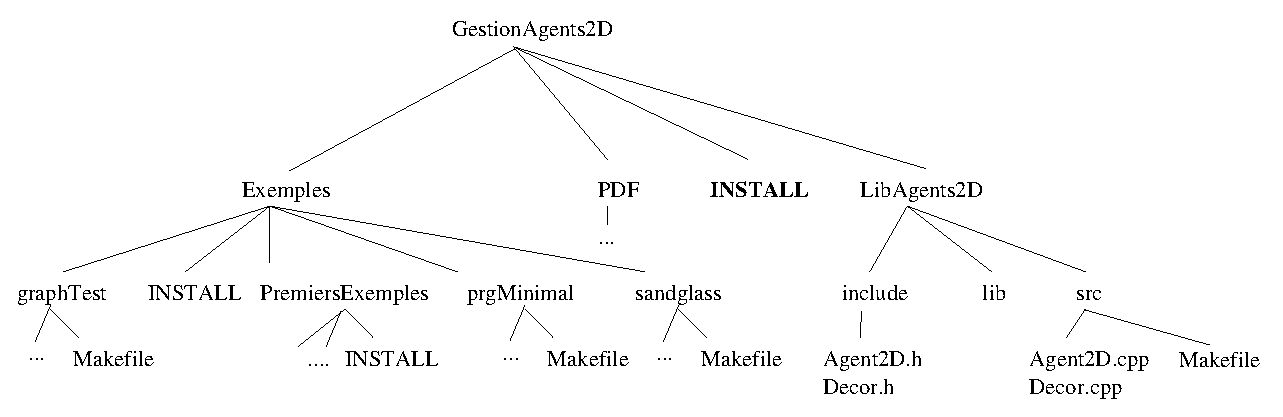
\includegraphics[width=15.5cm]{fig/arbo}
\end{center}
\caption{Description de l'arborescence de la biblioth\`eque}
\end{figure}

Aller dans le r\'epertoire {\tt LibAgents2D/src}
et faire {\tt \$ make}

Une biblioth\`eque {\tt libAgents2D.a} est alors plac\'ee dans le r\'epertoire
{\tt LibAgents2D/lib}

Des exemples de programmes sont disponibles dans le r\'epertoire
{\tt Exemples}.

\vspace{0.5cm}
{\bf ... mais on peut faire plus simple !}

\vspace{0.3cm}

En \'etant dans le r\'epertoire {\tt GestionAgents2D}, faire tout
simplement {\tt \$ ./INSTALL}

Il faut ensuite aller dans les r\'epertoires avec les divers exemples
et faire {\tt \$ make}\\
...mais on peut aussi faire {\tt \$ ./INSTALL}

\end{document}

